%!TEX root = ../../report.tex

\chapter{Simulation} % (fold)
\label{cha:simulation}
This chapter is meant to answer the questions what, why and how a simulator has been used in the framework.
Starts with a motivation section \ref{sec:sim_motivation} which defines the scope of the simulator
 in the project, followed by a comparison of simulators \ref{sec:sim_comparison_of_simulators} and how to define a robot and its environment in it \ref{sec:robot_definition}; in the next section \ref{sec:robot_creation} is explained how the simulation model of the legs has been created and how to add new features, whilst the creation of the environment is dealt in the section \ref{sec:environment_creation}; finishes with a how-to dedicated section for launching the simulation from scratch in \ref{sec:how_to_simulate}.
%!TEX root = ../../../report.tex
\section{Motivation} % (fold)
\label{sec:sim_motivation}
In the previous chapters the design of a human-proportional biped has been presented. 
The robot has been developed with security systems in both, software and hardware, that prolong the operating life of the robot. 
Nevertheless, every device in real life is prone to suffer damage which translates in to money and time for the user.
By forming part of the toolbox offered in the framework, a comprehensive biped simulation is given so the user can both work with the same algorithms in real and simulated life.

Whilst not being a complete replacement of the real life, it offers a similar experience what allows to do qualitative research.
As an example, neuronal networks or reinforcement learning algorithms, that learn by experience, can be developed faster in the simulator and then transfered to the real robot, reducing the workflow and the need of resources of the user and justifying its use.

A simulator consists basically of two elements: a physical engine and a graphical engine.
Whilst the first one is in charge of calculate all the physical interactions that the agent suffers, the second one offers the visual experience.
A congruent simulator with the presented framework will satisfy two conditions:
\begin{enumerate}
  \item The effort for testing among the simulation and real life must be minimized
  \item The results must be as closer to real life as possible. This includes multiphysics support (mechanical contacts, different aspects of tribology, wind, water...) but within a fair trade-off with computational speed.
\end{enumerate}

% section motivation (end)
%!TEX root = ../../../report.tex
\section{Comparison of simulators} % (fold)
\label{sec:sim_comparison_of_simulators}
When choosing a simulation platform there are several factors to have into account.
Three robotic simulators have been analyzed and compared. 
These are: LPZ Robots \cite{lpzrobots} (Figure \ref{fig:lpzrobots_example}), V-Rep \cite{vrep} (Figure \ref{fig:vrep_example}) and Gazebo \cite{gazebo} (Figure \ref{fig:gazebo_example}).
Some comparisons can be found in the literature as \cite{nogueiracomparative} or \cite{staranowicz2011survey} however the predominant criteria has been their integration with ROS.

\begin{figure}[hb!]
  \begin{subfigure}{.33\textwidth}
    \centering
    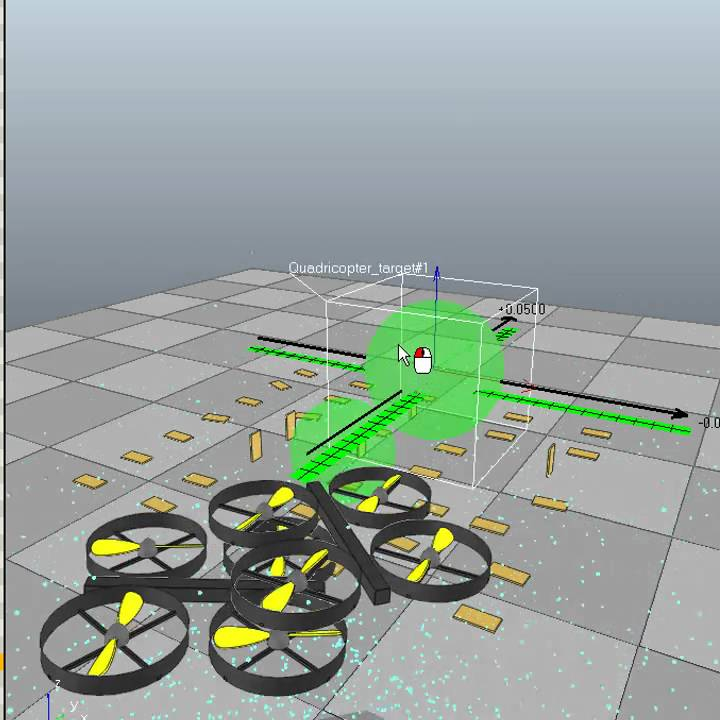
\includegraphics[width=.95\linewidth]{figures/vrep_example}
    \caption{V-Rep}
    \label{fig:vrep_example}
  \end{subfigure}%
  \begin{subfigure}{.33\textwidth}
    \centering
    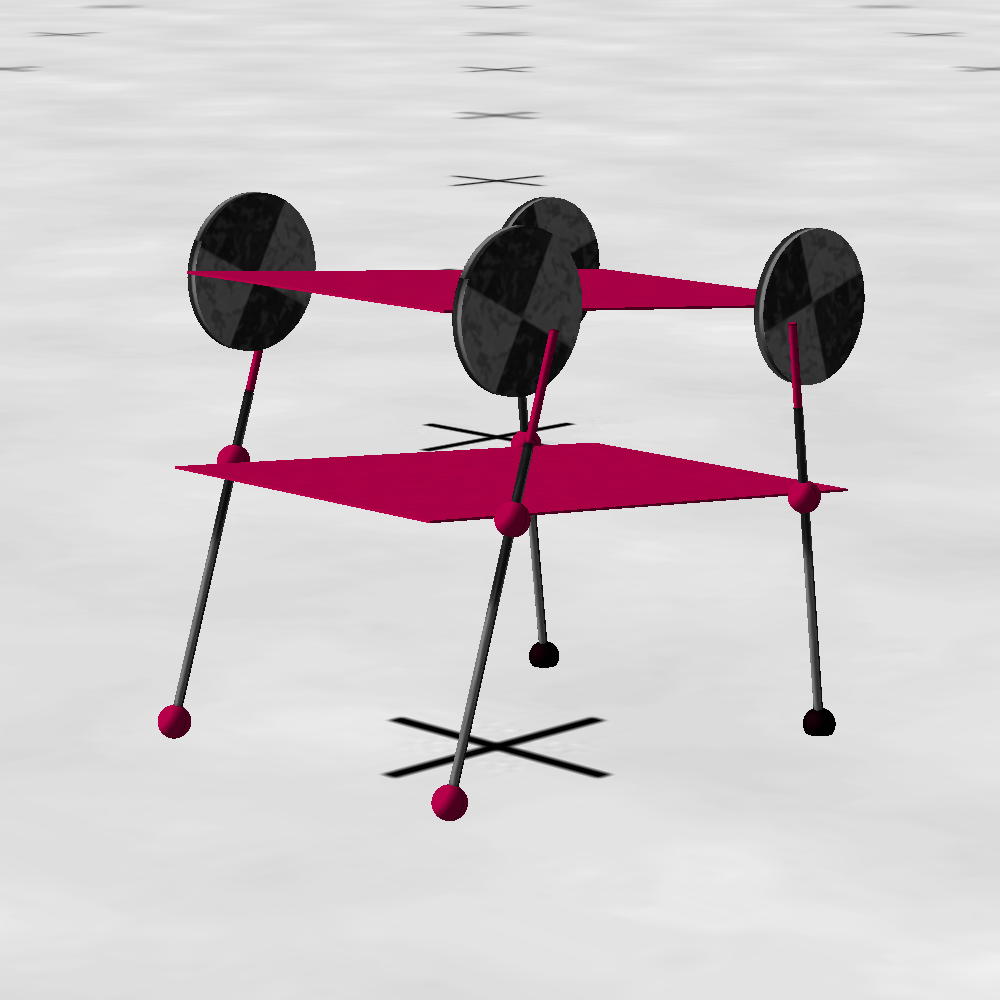
\includegraphics[width=.95\linewidth]{figures/lpzrobots_example}
    \caption{LPZ Robots}
    \label{fig:lpzrobots_example}
  \end{subfigure}
  \begin{subfigure}{.33\textwidth}
    \centering
    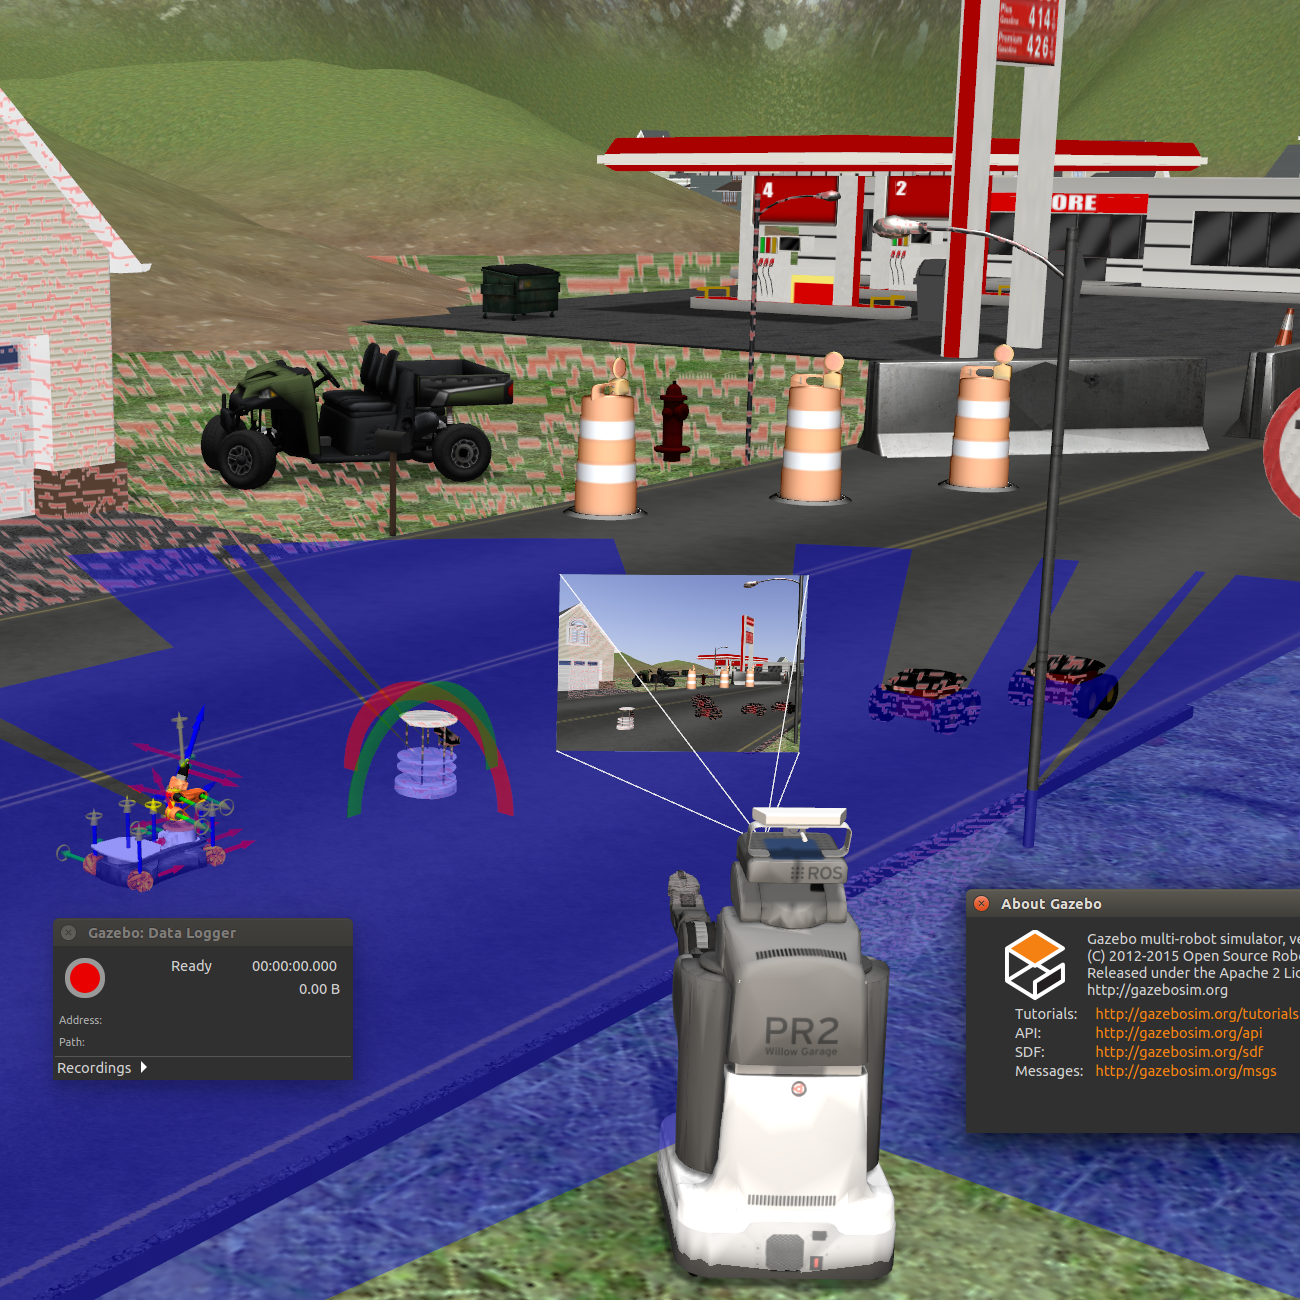
\includegraphics[width=.95\linewidth]{figures/gazebo_example}
    \caption{Gazebo}
    \label{fig:gazebo_example}
  \end{subfigure}
  \caption{Simulation examples of the software analyzed.}
  \label{fig:simulation_comparison}
\end{figure}

The RuBi robot is mainly targeted to be used in the AI department at the Maersk Mc-Kinney Møller Institute, where the toolbox GoRobots is being developed.
This is a set of tools, from a neuronal networks API to a genetic algorithm engine, written in C++ than is meant to be simulator-independent.
However, in order to provide a more general and supported simulation and development environment for the user, ROS Jade \cite{ros} has been selected as the tool to use.
The whole set of instruments provided in ROS along with its easy extendability give the opportunity to use the controllers and tools already developed in GoRobots.
Despite the fact that the three simulators compared have a C++ interface that would allow to interface them with ROS, Gazebo is already fully supported and integrated in ROS, making it the logic choice.
This reduces the learning curve of a new user and the installation process is easier due to it is included in the Open Source Robotics Foundation (OSRF) repositories.

Regarding the second condition, Gazebo has the feature of changing the physics engine in the beginning of the simulation, it has multiphysics support (fluids, electromagnetism...), it allows to load external geometries from STL or Collada and, the most important, has an active community behind it providing support and documentation. These are the reasons for selecting Gazebo as the simulator for the RuBi platform.
In \cite{physics_engine_gazebo_comparison}, a comparison with the different physical engines is carried out.
For the sake of simplicity the default one, Open Dynamics Engine (ODE), has been used, although the others have been tested.

% section comparison_of_simulators (end)\[
%!TEX root = ../../../report.tex
\section{Robot definition} % (fold)
\label{sec:robot_definition}
As in May of 2016, ROS Jade ecosystem has different formats to describe a robot.
These are SDF, URDF and Xacro.
At some point they are all transformed to a unique sort of format but the decision of how to express the robot for the simulation is needed from the beginning.


\begin{enumerate}
  \item \textbf{URDF \footnote{http://wiki.ros.org/urdf}}: is an open standard used in all the simulators mentioned or others like RobWork \cite{robwork}. 
  It allows to define all the properties of a single robot but lacks other which are important when simulating. 
  It is mainly used for visual representations or schematic robot definitions.
  \item \textbf{Xacro \footnote{http://wiki.ros.org/xacro}}: is a parametric format that easy the writing of the URDF.
  It allows logic conditions like \textit{if, for} and from ROS Jade any virtual python condition.
  This code is then compiled into a URDF automatically which give Xacro complete interoperability with URDF readers.
  \item \textbf{SDF \footnote{http://sdformat.org}}: adapted to the current requirements of the simulation environments.
  With it can be defined from \textit{worlds} to air properties in the case or UAV simulations.
\end{enumerate}

Despite SDF contains more information, there are several tools in ROS Jade that make use of URDF.
Two of them are RViz and ROS Control, explained in the section \ref{sub:ros_control}.
As this last one is a pillar of the framework itself, the decision of making use of URDF as format for describing the robot was taken.
However, the robots developed have been written in Xacro due to the tools that easy the coding of the robot.
% section robot_definition (end)
%!TEX root = ../../../report.tex
\section{Robot creation} % (fold)
\label{sec:robot_creation}
One of the goals of the framework is to easy its continuity, thus this section is dedicated to explain how the robot was created.

A robot is defined as a set of links jointed.
A link contains at least three blocks of information:
\begin{enumerate}
   \item The collision model: used to calculate the collisions with other agents in the simulation.
   \item The visual model: uniquely used for visual purposes.
   \item The inertial information: defines physical properties like the mass and the moments of inertia of the link.
\end{enumerate} 

A trade-off must be found for the precision of the collision model between accuracy and speed.
The more detailed is the model, the higher will be computation time which translates into more accuracy and more computation time.
The general advice is to have two simulation models: one for visual purposes and the other one for collisions.

In the case of the links of presented robot, the visual models are obtained directly by exporting the parts from SolidWorks whilst the collision models are made of primitive gazebo shapes (cubes, cylinders, spheres...) for the whole body but the feet.
Due to the robot is not meant to hit anything, the possible collisions in the body are not a priority, then each link is represented as a cylinder of the same length of the CAD model and of a radius enough to cover the whole part.
An example can be seen in the figure \ref{fig:collision_model}.

The moments of inertia of each individual link are obtained directly from SolidWorks.
The CAD model includes the materials and thus the masses.
From these, the program is able to calculate the moments of inertia.
The figure \ref{fig:moments_of_inertia} shows the representation of these in the simulation.


\begin{figure}[hb!]
  \centering
  \begin{subfigure}{.45\textwidth}
    \centering
    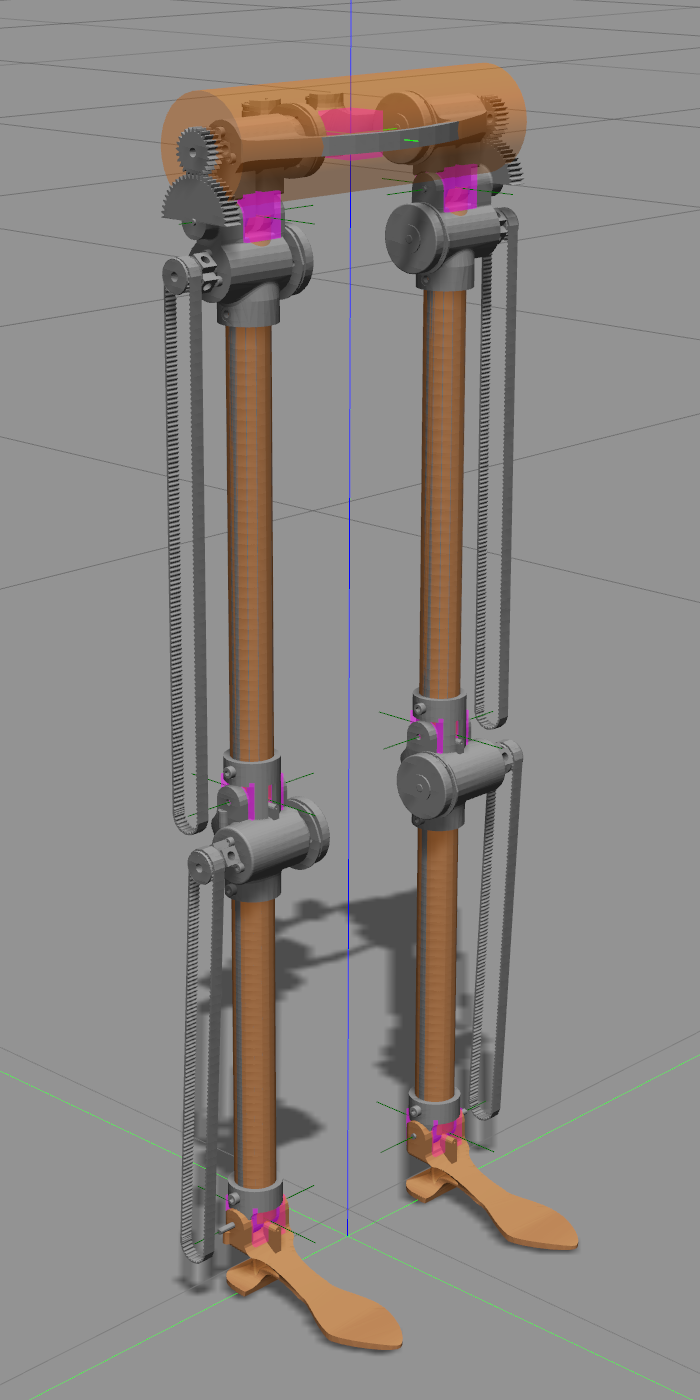
\includegraphics[width=.5\linewidth]{figures/gazebo_collision_model.png}
    \caption{Gazebo showing the visual model, the moments of inertia and the collision model}
    \label{fig:collision_model}
  \end{subfigure}
  \begin{subfigure}{.45\textwidth}
    \centering
    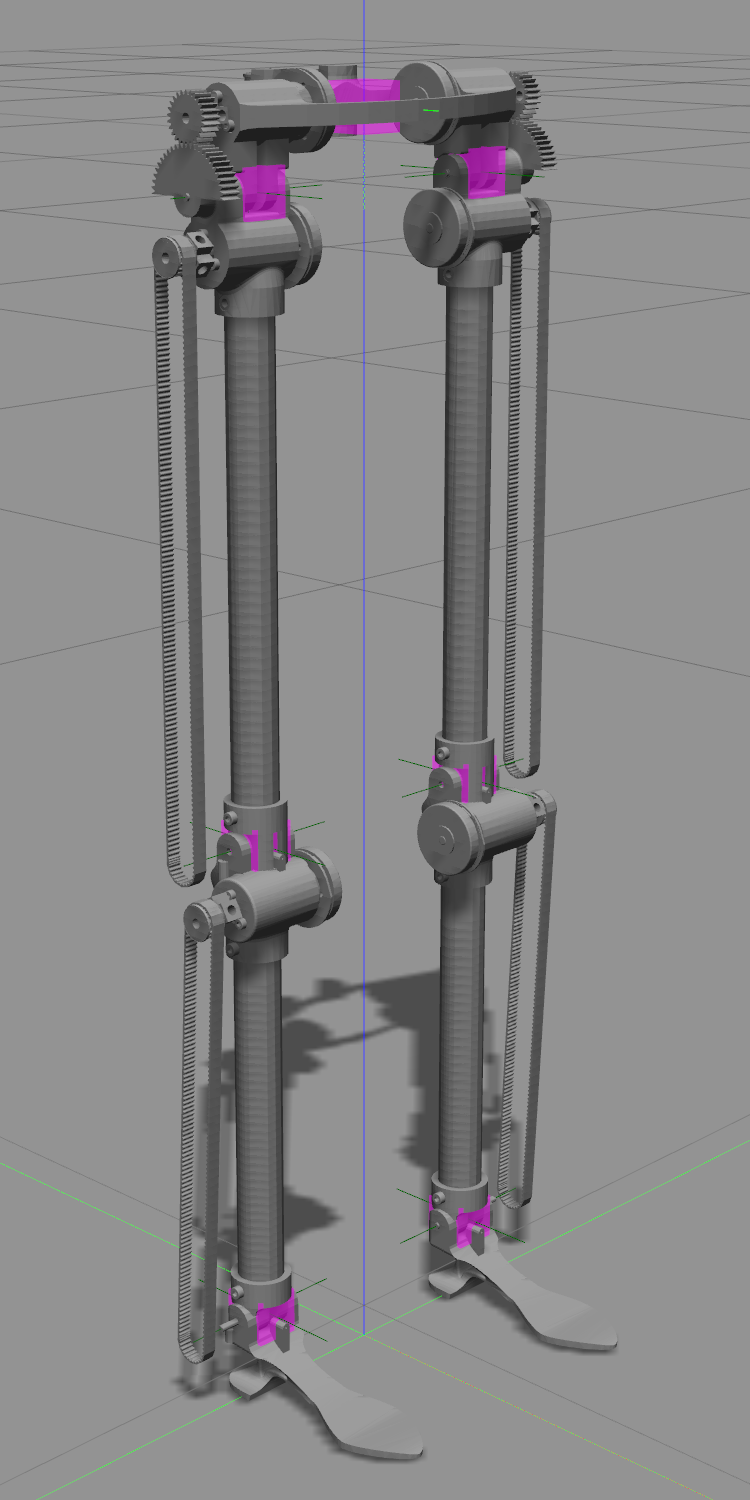
\includegraphics[width=.5\linewidth]{figures/gazebo_intertia_moments.png}
    \caption{Gazebo showing the visual model and the moments of inertia}
    \label{fig:moments_of_inertia}
  \end{subfigure}
\end{figure}

It is important to notice that the visual models and moments of inertia have been exported from the correct coordinate system.
In the case of the ankle, for example, the STL file and the moments of inertia are calculated from the coordinate system positioned in the middle of the rotational axis of the ankle, pointing the Z axis to the rotational axis and Y to the biggest extension of the part.
This can be seen in the figure \ref{fig:solidworks_ankle_coodinate_system}.

\begin{figure}[ht!]
  \centering
  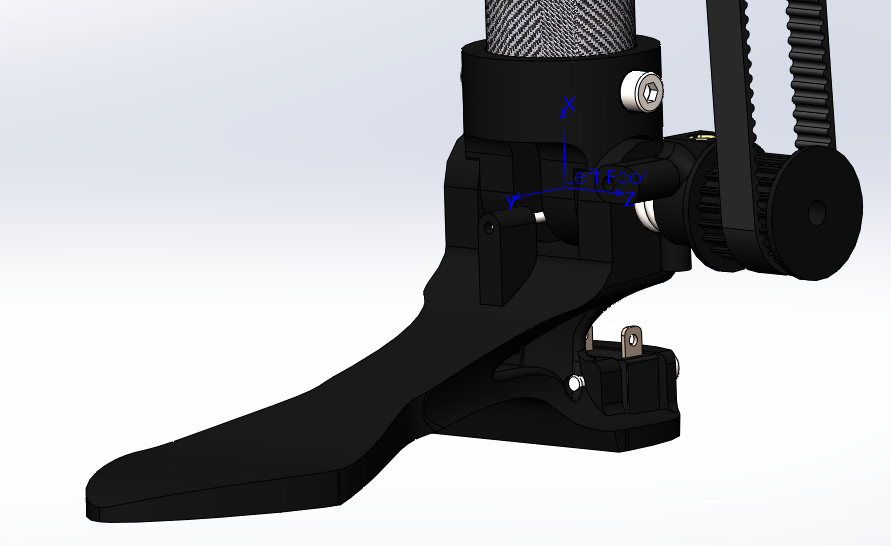
\includegraphics[width=0.75\linewidth]{figures/solidworks_ankle_coordinate_system}
  \caption{Coordinate system of the left ankle in SolidWorks}
  \label{fig:solidworks_ankle_coodinate_system}
\end{figure}

Finally, in the Xacro file the information that lacks the URDF must be added in order to simulate with Gazebo.
Eventually, to the RuBi description is added:
\begin{enumerate}
  \item \textbf{Plug-in for ROS Control}: Offers an interface for using ROS Control inside Gazebo.
  \item \textbf{Contact sensors}: Simulates contact sensors as in the feet of the real robot.
  \item \textbf{Defines friction of the components}: as the friction between the feet and the floor.
\end{enumerate}

% section robot_creation (end)
%!TEX root = ../../../report.tex
\section{Environment creation} % (fold)
\label{sec:environment_creation}
Besides the robot, other elements can be added to the simulated world.
From the Gazebo database, other robot models or parts (as a beer or a brick) can be inserted and used for any kind of experiments.

\begin{figure}[hb!]
  \centering
  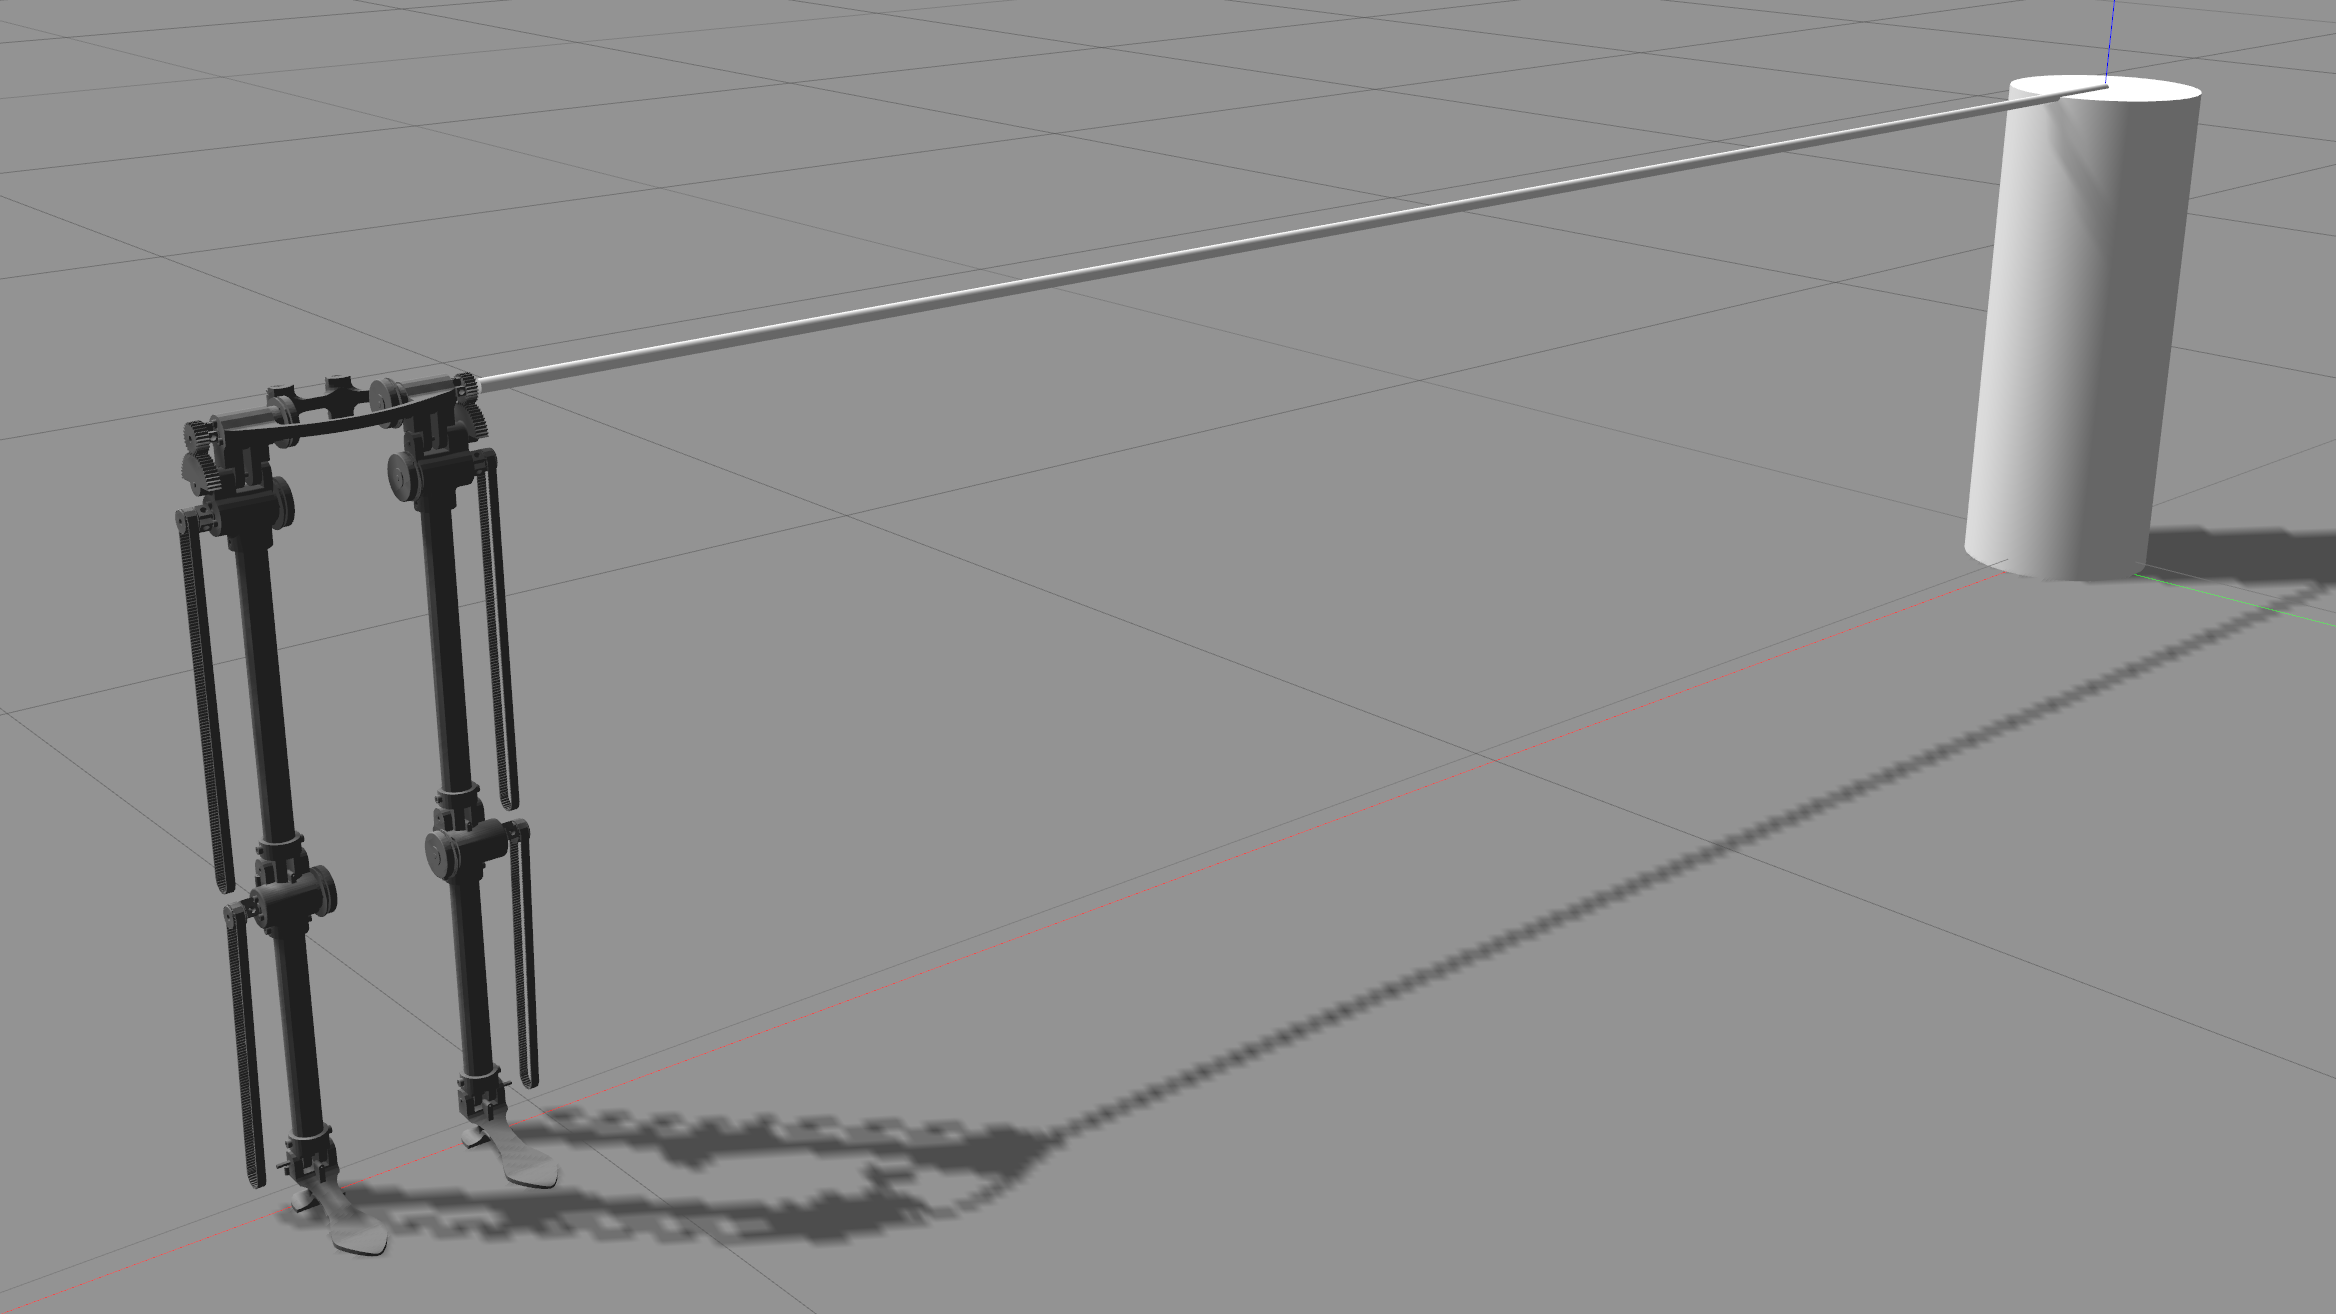
\includegraphics[width=0.75\linewidth]{figures/gazebo_rotational_holder}
  \caption{Rotational robot holder and robot}
  \label{fig:rotational_robot_holder}
\end{figure}

\hfill

In the final framework an extra tool is provided: a rotational robot holder.
It is inspired in the DACbot simulation environment in LPZ Robots, being fully parametric and reducing the degrees of freedom of the robot to constraint its motion to the scenario under study.
It can be seen in Figure \ref{fig:rotational_robot_holder}.

% section environment_creation (end)
%!TEX root = ../../../report.tex
\section{How to simulate} % (fold)
\label{sec:how_to_simulate}
The actions for starting the simulation are minimal and, with everything installed, just a terminal shall be opened and the user have to insert:

\begin{lstlisting}
roslaunch legs_gazebo legs_world.launch
\end{lstlisting}

The launch file will load ROS Control along with the simulation.
From that moment the user can run the controllers and the legs will move equally than in the real robot.
% section how_to_simulate (end)

% chapter simulation (end)
